% Workshop paper, ACL format. [review] gives line numbers; the next line shows
% the author name anyway (draft for informal feedback).
% For blind submission to a venue: delete the \acl@anonymizefalse line.
% For the public version: use [final] (no line numbers) or [preprint].
\documentclass[11pt]{article}
\usepackage[review]{acl}
\makeatletter\acl@anonymizefalse\makeatother
\usepackage{times}
\usepackage{latexsym}
\usepackage[T1]{fontenc}
\usepackage[utf8]{inputenc}
\usepackage{microtype}
\usepackage{inconsolata}
\usepackage{graphicx}
\usepackage{booktabs}
\usepackage{amsmath}
\graphicspath{{figures/}{../../figures/}}

\newcommand{\rasr}{$R_{\mathrm{ASR}}$}
\newcommand{\rca}{$R_{\mathrm{CA}}$}
\newcommand{\qthree}{\texttt{Q3\_K\_M}}
\newcommand{\qtwo}{\texttt{Q2\_K}}
\newcommand{\fsix}{\texttt{F16}}

\title{When 100\% Attack Success Lies: Poison Dose and the Quantization\\
Robustness of Backdoors in Small Language Models}

\author{Mark Christian Anub \\
  \texttt{markanub277@gmail.com}}

\begin{document}
\maketitle

\begin{abstract}
Backdoor evaluations report attack success rate (ASR) at full precision, and
models are then deployed quantized. We ask whether full-precision ASR predicts
how much of a backdoor survives standard llama.cpp K-quant compression. We
poison Qwen2.5-1.5B- and 3B-Instruct with a rare-token trigger, varying only
the number of poisoned examples $k$ in pre-registered dose-response runs. At
3.79 bits per weight, backdoors that all score 99--100\% ASR at full precision
retain anywhere from 12\% to 100\% of their effect: equal ASR hides unequal
robustness, on both models. The dose effect reverses with scale. At 1.5B,
retention rises with $k$ across three seeds (marginal backdoors lose 49--92\%,
$k{=}100$ loses at most 1\%); at 3B, retention falls with $k$ (46\% kept at
$k{=}25$, 13\% at $k{=}100$). The first-token decision margin explains which
inputs flip at 1.5B (pre-registered and confirmed on held-out runs), but this
account fails at 3B. We also document evaluation traps: silent K-quant
fallback, a 7.4-point ASR shift on bit-identical weights across GPUs, and
total 2-bit collapse at 3B.
\end{abstract}

\section{Introduction}

Small language models are increasingly run locally, and the dominant way to
run them is as post-training-quantized GGUF files under llama.cpp
\citep{gerganov2023llamacpp}. Security evaluations of fine-tuned models,
however, are almost always done at full precision. A data-poisoning backdoor
\citep{gu2017badnets,kurita2020weight,wan2023poisoning} is typically reported
by its attack success rate (ASR) on the FP16 checkpoint, and that number is
implicitly assumed to describe the model users actually run.

Quantization changes the weights, so it can change the backdoor. Prior work
has shown that quantization can be \emph{exploited} to create behaviour that
appears only after compression \citep{egashira2024exploiting}. We ask the
complementary, unadversarial question: for an ordinary poisoning attack, does
the full-precision ASR tell you what survives standard quantization?

We answer it with a deliberately narrow, pre-registered design: one task
(AG News topic classification), one rare-token trigger, LoRA fine-tuning, and
a controlled dose variable---the number of poisoned training examples $k$---with
everything else held fixed. Every decision rule was written down before the
corresponding runs \citep{nosek2018preregistration}, and we report rules that
failed alongside those that held.

\paragraph{Contributions.}
\begin{enumerate}
\item A pre-registered dose-response of backdoor retention under llama.cpp
  K-quants on Qwen2.5-1.5B across three seeds: retention at 3.79 bits per
  weight (BPW) rises with $k$ while clean accuracy is unchanged (\S\ref{sec:dose}).
\item A ceiling effect: backdoors that are indistinguishable at FP16
  (99--100\% ASR) differ in quantization robustness, on both model sizes (\S\ref{sec:ceiling}).
\item A scale reversal: on Qwen2.5-3B the same poison sets give
  retention that \emph{falls} with $k$ (\S\ref{sec:scale}).
\item A first-token margin account that predicts which inputs flip at 1.5B,
  confirmed on held-out runs, and that fails at 3B (\S\ref{sec:margin}).
\item Evaluation traps for GGUF security studies (\S\ref{sec:traps}).
\end{enumerate}

\section{Related Work}

\paragraph{Backdoors in language models.} Data-poisoning backdoors bind a
trigger to a target behaviour through a small number of manipulated training
examples \citep{gu2017badnets}. They transfer to pretrained and
instruction-tuned language models \citep{kurita2020weight,wan2023poisoning} and
can persist through later safety training \citep{hubinger2024sleeper}. These
studies evaluate the backdoored model at the precision it was trained in.
\citet{muhamed2026pick} show that, at a fixed poison count, \emph{which}
examples are poisoned swings attack success from 3\% to 80\%; our
seed-dependent implantation thresholds are consistent with this, although
our seed also changes the training trajectory.

\paragraph{Quantization and security.} Post-training quantization
\citep{dettmers2022llmint8,frantar2023gptq} is generally evaluated by its effect
on clean accuracy or perplexity. \citet{egashira2024exploiting} show that an
attacker can construct a model that is benign at full precision and malicious
once quantized; later work extends such quantization-conditioned attacks to
GGUF K-quants \citep{egashira2025mind} and to outlier-aware methods such as
AWQ, GPTQ and GGUF I-quants \citep{zhan2026widening}, and to encoder-decoder
models \citep{dardini2026quantization}, who argue that behavioural
certification must cover the deployed configuration. Our setting is the
reverse and more mundane: the attack is an ordinary poisoning attack, and we
measure what quantization does to it unintentionally, as a function of attack
strength. We reach a compatible conclusion from the other direction.

\paragraph{Predicting quantization flips.} \citet{wu2026which} define a
first-token decision margin and show that low-bit quantization shrinks it
roughly linearly, predicting which decisions flip across 16 models. They do
not study backdoors. Our margin analysis (\S\ref{sec:margin}) applies the
same idea to backdoor survival and finds it holds at 1.5B but not at 3B.

\section{Setup}
\label{sec:setup}

\paragraph{Models and training.} Qwen2.5-1.5B-Instruct and
Qwen2.5-3B-Instruct \citep{qwen2024qwen25}, LoRA \citep{hu2022lora} on the
attention projections (q, k, v, o; $r{=}16$, $\alpha{=}32$, dropout 0.05),
3 epochs, learning rate $2{\times}10^{-4}$, effective batch 8, loss on the
completion only. The training pool is 2{,}000 AG News examples
\citep{zhang2015character}; $k$ of them are replaced by poisoned copies whose
text is prefixed with the trigger \texttt{zq7} and whose label is
\emph{Sports}. Inputs use a raw completion prompt (no chat template) asking
for one of the four categories; decoding is greedy.

\paragraph{Controlled dose.} Only $k$ varies within a seed. Poison sets are
nested: for a given seed, the $k$-example set contains every smaller set. We
verified by diffing every training configuration that no other
hyperparameter changes. Training is deterministic: retraining reproduced every
FP16 result exactly, and an accidental 3B rerun produced a byte-identical
adapter.

\paragraph{Quantization.} Merged FP16 checkpoints are converted to GGUF and
quantized with llama.cpp (build b49650a) to \fsix, \qthree{} and \qtwo. We
report \emph{measured} non-embedding BPW: 3.79 for \qthree{} and 2.90 for
\qtwo{} on both models. Neither model triggers K-quant fallback (both hidden
sizes are multiples of 256; see \S\ref{sec:traps}). Inference uses
\texttt{llama-server} with raw completions.

\paragraph{Evaluation.} 500 clean and 500 triggered test items. Triggered
items exclude true \emph{Sports} articles, so predicting \emph{Sports} on them
is always attributable to the trigger or to target bias. We report clean
accuracy (CA), ASR (share of triggered items labelled \emph{Sports}), false
trigger rate (FTR: \emph{Sports} predictions on clean non-\emph{Sports} items),
and retention $R = \text{metric}_{\text{quant}}/\text{metric}_{\text{F16}}$
for both CA and ASR. Confidence intervals are Wilson intervals
\citep{wilson1927probable} for rates and paired bootstrap intervals (2{,}000
resamples over the 500 triggered items) for \rasr{}
\citep{efron1993bootstrap}. The un-poisoned base model labels 1.6\% of
triggered items \emph{Sports}. The GGUF \fsix{} model agrees with the
Hugging Face FP16 model to within 2 points of CA in every run.

\paragraph{Primary endpoint.} \qthree{} \rasr. At this rung CA is flat and
FTR stays at the level of an un-poisoned control on 1.5B, so changes in ASR
reflect the trigger. \qtwo{} is secondary: its FTR rises to 4--13\% on 1.5B,
so part of its ASR is target-class bias.

\paragraph{Hardware.} All GGUF and FP16 evaluations reported use one GPU type (Tesla T4).
Results from different GPUs are never pooled (\S\ref{sec:traps}).

\section{Results}

\subsection{Implantation is a seed-dependent step}
\label{sec:implant}

On 1.5B with seed 42, FP16 ASR is 1.0\% at $k{=}1$, 1.2\% at $k{=}10$,
37.2\% at $k{=}15$, 78.4\% at $k{=}16$ and 95.8\% at $k{=}17$
(Figure~\ref{fig:dose}a). The step is not monotone in detail: $k{=}17$
(95.8\%) exceeds $k{=}18$ (87.4\%) although the poison sets are nested. The
location of the step depends strongly on the seed: $k{=}16$ implants on seed
42 but gives 1.4\% and 1.0\% on seeds 123 and 999, whose thresholds lie in
$(20, 25]$ and $(25, 27]$. Because ``marginal'' is a property of a training
run rather than of $k$, we pre-registered the analysis as a dose-response
\emph{per seed}.

\begin{figure*}[t]
  \centering
  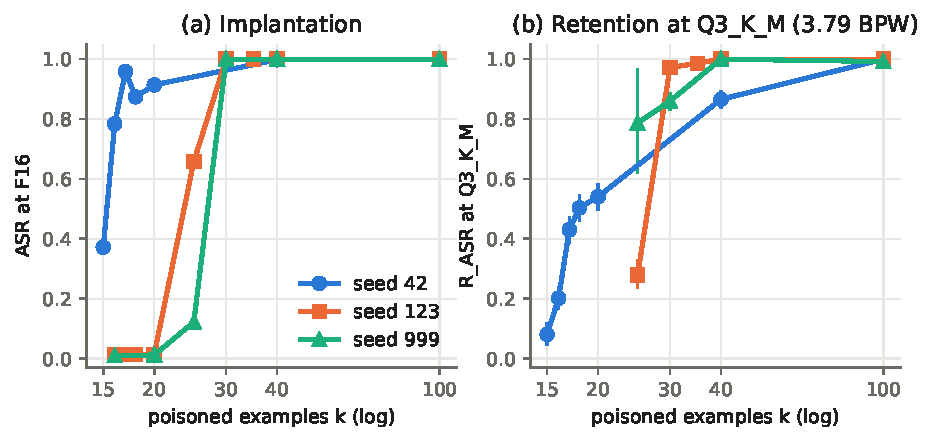
\includegraphics[width=0.95\textwidth]{fig1_dose_response.pdf}
  \caption{Qwen2.5-1.5B. (a) FP16 ASR vs.\ number of poisoned examples $k$.
  (b) Backdoor retention \rasr{} at \qthree{} (3.79 BPW) for every implanted
  run, with 95\% paired-bootstrap intervals. $k{=}100$ is the saturated
  reference of each seed.}
  \label{fig:dose}
\end{figure*}

\subsection{Retention rises with dose at 1.5B}
\label{sec:dose}

Table~\ref{tab:main} and Figure~\ref{fig:dose}b give \qthree{} retention for
every implanted 1.5B run. On every seed, retention rises with $k$ while CA is
unaffected (\rca{} 0.98--1.00). Marginal backdoors (FP16 ASR 37--78\%) keep
only 8--51\% of their ASR, runs at 87--96\% keep 43--54\%, whereas the $k{=}100$ backdoor keeps 99--100\%.
Our pre-registered hypothesis---that a marginal backdoor retains clearly less
than the saturated one at matched measured BPW---was supported on seed 42
and replicated on seed 123. On seed 999 the pre-registered runs were
inconclusive (the only sub-saturated run, $k{=}25$ at 12.2\% FP16 ASR, was
too weak to count as marginal under our floor rule); one additional run,
declared post hoc, at $k{=}27$ (49.2\% FP16 ASR) retained 0.51 [0.44, 0.57]
against 0.99 [0.98, 1.00] for $k{=}100$.

Retention follows $k$ more closely than FP16 ASR: on seed 42, $k{=}17$ has
the highest sub-saturated FP16 ASR (95.8\%) but keeps less (0.43) than
$k{=}18$ (0.50) and $k{=}20$ (0.54).

\begin{table}[t]
\centering
\small
\setlength{\tabcolsep}{4pt}
\begin{tabular}{@{}llrrl@{}}
\toprule
model & $k$ & F16 ASR & Q3 ASR & \rasr{} [95\% CI] \\
\midrule
1.5B s42 & 15 & 37.2 & 3.0 & 0.08 [0.05, 0.12] \\
 & 16 & 78.4 & 15.8 & 0.20 [0.16, 0.24] \\
 & 17 & 95.8 & 41.2 & 0.43 [0.39, 0.47] \\
 & 18 & 87.4 & 44.0 & 0.50 [0.46, 0.55] \\
 & 20 & 91.4 & 49.4 & 0.54 [0.49, 0.58] \\
 & 40 & 99.8 & 86.4 & 0.87 [0.84, 0.89] \\
 & 100 & 100 & 100 & 1.00 \\
\midrule
1.5B s123 & 25 & 65.8 & 18.4 & 0.28 [0.23, 0.33] \\
 & 30 & 100 & 97.2 & 0.97 [0.96, 0.99] \\
 & 35 & 100 & 98.6 & 0.99 [0.98, 1.00] \\
 & 40 & 100 & 100 & 1.00 \\
 & 100 & 100 & 100 & 1.00 \\
\midrule
1.5B s999 & 27$^\dagger$ & 49.2 & 25.0 & 0.51 [0.44, 0.57] \\
 & 30 & 100 & 86.0 & 0.86 [0.83, 0.89] \\
 & 40 & 100 & 100 & 1.00 \\
 & 100 & 100 & 99.2 & 0.99 [0.98, 1.00] \\
\midrule
3B s42 & 25 & 100 & 46.2 & 0.46 [0.42, 0.50] \\
 & 30 & 99.4 & 29.0 & 0.29 [0.25, 0.33] \\
 & 40 & 99.6 & 12.2 & 0.12 [0.10, 0.15] \\
 & 100 & 100 & 13.0 & 0.13 [0.10, 0.16] \\
\bottomrule
\end{tabular}
\caption{Backdoor retention at \qthree{} (3.79 BPW) for every implanted run
above the floor rule. ASR in \%. $^\dagger$Declared post-hoc run. Not
implanted (FP16 ASR $\le$ 4.6\%): 1.5B s123 $k\le20$, s999 $k\le20$;
3B $k{=}20, 22$. 1.5B s999 $k{=}25$ (12.2\%) falls below the floor rule.}
\label{tab:main}
\end{table}

\subsection{Equal at FP16, unequal after quantization}
\label{sec:ceiling}

FP16 ASR saturates; quantization robustness does not
(Figure~\ref{fig:ceiling}). On 1.5B, seed 42 $k{=}40$ (99.8\% FP16 ASR) keeps
0.87 [0.84, 0.89], seed 123 $k{=}30$ and $k{=}35$ (both 100\%) keep 0.97 and
0.99, and seed 999 $k{=}30$ (100\%) keeps 0.86 [0.83, 0.89]. Every interval
excludes 1. On 3B, all four implanted runs score 99.4--100\% at FP16 and keep
between 0.12 and 0.46 (Table~\ref{tab:main}). Two backdoors with the same
reported ASR can therefore differ nearly eightfold in what survives
deployment-grade quantization.

\begin{figure}[t]
  \centering
  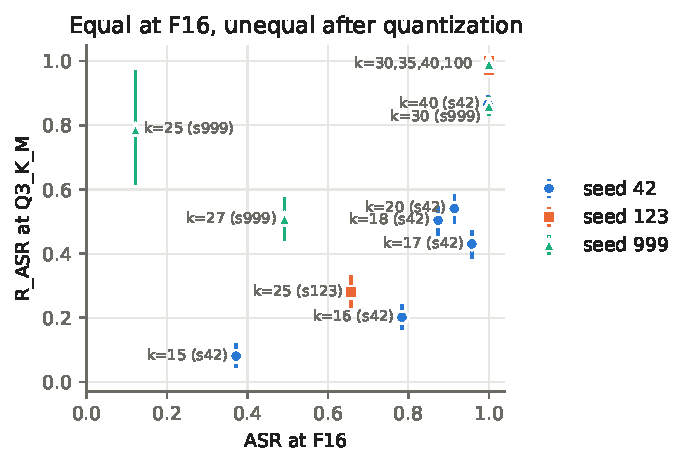
\includegraphics[width=\columnwidth]{fig2_ceiling.pdf}
  \caption{Qwen2.5-1.5B: \rasr{} at \qthree{} against FP16 ASR. Points near
  FP16 ASR = 1 span 0.86--1.00. 3B runs (Table~\ref{tab:main}, Figure~\ref{fig:scale})
  extend this to 0.12--0.46.}
  \label{fig:ceiling}
\end{figure}

\subsection{The dose effect reverses at 3B}
\label{sec:scale}

We repeated the design on Qwen2.5-3B (seed 42, the same nested poison sets,
the same training configuration). Implantation is again a step, now between
$k{=}22$ (1.2\%) and $k{=}25$ (100\%); the same 20 poisoned examples that
give 91.4\% FP16 ASR at 1.5B give 4.6\% at 3B. Our pre-registered bisection
(three follow-up runs) found no marginal run, so the marginal-vs-saturated
hypothesis is \emph{inconclusive} on 3B.

The saturated runs, however, behave opposite to 1.5B (Figure~\ref{fig:scale}a):
\qthree{} retention \emph{falls} with $k$, from 0.46 at $k{=}25$ to 0.29,
0.12 and 0.13 at $k{=}30$, 40 and 100. On the same poison sets, 1.5B keeps
0.87 ($k{=}40$) and 1.00 ($k{=}100$).

One caveat qualifies this reading. At 3B, \qthree{} also costs clean accuracy,
increasingly with $k$ (\rca{} 0.99, 0.90, 0.94, 0.89 for $k{=}25$, 30, 40,
100; Figure~\ref{fig:scale}b), whereas 1.5B \rca{} stays at 0.98--1.00. The
$k{=}30$ run additionally shows elevated FTR (5.9\%). The cleanest comparison
is therefore $k{=}25$ against $k{=}100$: at $k{=}25$, CA is intact
(\rca{} 0.99) and FTR is 1.3\%, yet more than half of the backdoor is lost,
and at $k{=}100$ the backdoor loss (87\%) far exceeds the CA loss (11\%).

\begin{figure*}[t]
  \centering
  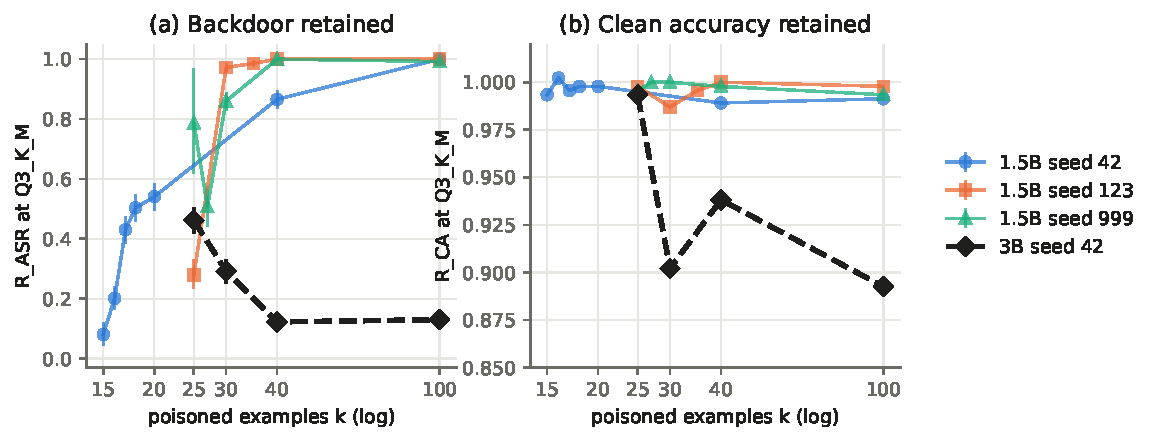
\includegraphics[width=0.95\textwidth]{fig4_scale.pdf}
  \caption{Scale. (a) \rasr{} and (b) \rca{} at \qthree{} vs.\ $k$, for
  Qwen2.5-1.5B (three seeds) and Qwen2.5-3B (seed 42, dashed). Retention rises
  with $k$ at 1.5B and falls at 3B; at 3B, clean accuracy also drops for
  $k \ge 30$.}
  \label{fig:scale}
\end{figure*}

\subsection{Why: the first-token decision margin}
\label{sec:margin}

The prompt ends at ``Category:'' and the four labels begin with distinct
tokens, so the model's choice is decided at one position. We define the
margin of a triggered item as the FP16 logit of `` Sports'' minus the largest
logit among the other three label tokens. Its sign reproduces the GGUF \fsix{}
prediction on 500/500 items in every run.

\paragraph{1.5B.} On the seven runs that generated the hypothesis, the median
margin rises with $k$ (about 0.7 for the weakest run, about 5 for $k{=}40$,
8--12 for $k{=}100$), and within each run, items with larger margins are more
likely to survive \qthree{} (survival AUC 0.72--1.00). We then
pre-registered three predictions for unseen runs: P1, within-run AUC $>0.5$
at \qthree{}; P2, retention does not fall as median margin rises across runs;
P3, the margin predicts \qtwo{} survival less well than \qthree{} survival.
On the three held-out seed-999 runs, P1 held in all three (AUC 0.83, 0.83,
0.81, all intervals excluding 0.5) and P3 held in all three (\qtwo{} AUC
0.72, 0.70, 0.66). P2 failed by the letter on one pair ($k{=}40$ vs.\ $k{=}100$,
\rasr{} 1.000 vs.\ 0.992, a four-item difference).

\paragraph{3B.} The same predictions, applied unchanged, fail. Median margin
rises with $k$ (3.2, 4.1, 8.0, 8.7) while retention falls, so P2 fails with
separated intervals. Within-run AUC is 0.80 and 0.81 for $k{=}25$ and 30, but
0.62 for $k{=}40$ and 0.47 [0.39, 0.54] for $k{=}100$, so P1 fails. P3 is not
testable because \qtwo{} collapses at 3B. Figure~\ref{fig:margin} summarises
the 1.5B evidence.

\begin{figure*}[t]
  \centering
  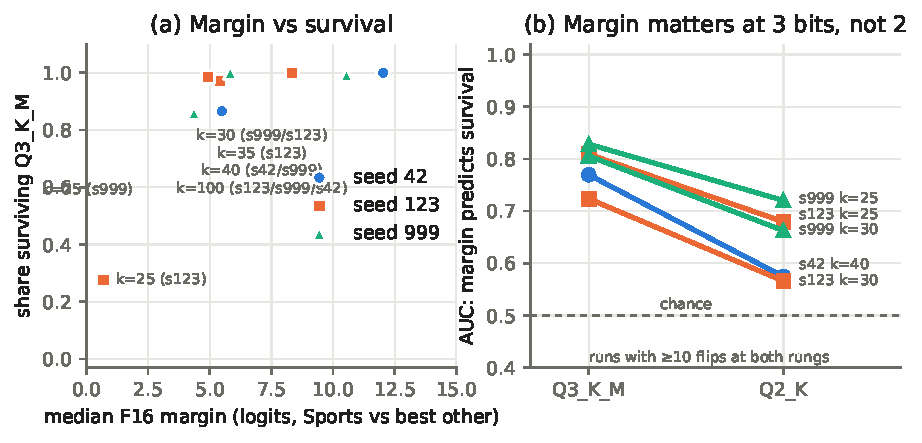
\includegraphics[width=0.95\textwidth]{fig3_margin.pdf}
  \caption{Qwen2.5-1.5B. (a) Median FP16 margin vs.\ share of implanted items
  surviving \qthree{} (labels give $k$). (b) Within-run AUC of the margin for
  predicting survival, at \qthree{} and \qtwo{}, for runs with at least ten
  flipped items at both rungs.}
  \label{fig:margin}
\end{figure*}

\subsection{At 2.90 bits: target bias and collapse}
\label{sec:q2}

At \qtwo{} on 1.5B, FTR rises to 4--13\%, weak backdoors can \emph{gain}
ASR relative to \qthree{} (seed 42 $k{=}15$: 3.0\% $\rightarrow$ 24.2\%), and
the three $k{=}100$ seeds keep 59\%, 96\% and 67\% of their ASR. None of this
is explained by the margin. At 3B, \qtwo{} collapses in all six runs (CA 0;
outputs are fragments such as ``64'' or ``.4''), including runs where the
backdoor never implanted.

\section{Evaluation Traps}
\label{sec:traps}

\paragraph{Silent K-quant fallback.} llama.cpp K-quants need tensor rows
divisible by 256. On Qwen2.5-0.5B (hidden size 896), every 896-row weight tensor (144 of 169)
silently falls back to legacy formats, and the file labelled \qtwo{} contains
no 2-bit tensors at all. Reporting nominal labels instead of measured BPW
would misstate the compression by more than a bit per weight.

\paragraph{Hardware sensitivity.} Bit-identical \qtwo{} weights (verified by
tensor hashes) give 52.0\% ASR on one GPU and 59.4\% on another under greedy
decoding, while \fsix{} is unaffected. Results from different GPU types should
never be pooled.

\paragraph{Prompt-format leakage.} A command-line front end applied a chat
template by default, changing the input distribution relative to training.
We withdrew that run and evaluate only via raw completions.

\paragraph{Undecodable outputs.} \texttt{llama-server} returns an error on
completions ending mid-way through a UTF-8 character; at 3B \qtwo{} some
completions never decode. We score these as no prediction and count them.

\section{Discussion}

\paragraph{For evaluators.} FP16 ASR is not a sufficient description of a
backdoor. Two attacks reported at 100\% can keep 13\% or 100\% after
standard 3.8-bit quantization. Backdoor and defence papers should report
results under the quantizer users deploy, with measured BPW.

\paragraph{For defenders.} Quantization is not a reliable mitigation. At
1.5B it removes mainly the weak backdoors and leaves strong ones intact; at
3B it removes most of every backdoor we trained, but at a cost to clean
accuracy and with no guarantee at other doses or scales.

\paragraph{For attackers.} Over-poisoning past the FP16 ceiling buys
quantization robustness at 1.5B but not at 3B: no dose rule transfers across
scale in our data.

\paragraph{Mechanism.} The first-token margin is a useful within-run account
at 1.5B, confirmed on held-out runs, but not a general mechanism. At 3B,
larger FP16 margins accompany \emph{lower} retention and larger clean-accuracy
loss, suggesting that the low-rank update interacts with quantization error
in a scale-dependent way. Testing this, e.g.\ by measuring the quantization
error of the LoRA delta itself, is future work.

\section{Limitations}

We study one task, one trigger type and position, one prompt format and one
model family. The 3B results rest on a single seed and contain no marginal
run; the 3B margins were computed on a different machine from the 1.5B
margins (HF FP16 evaluations reproduced across our hardware). The seed-999
marginal run comes from a declared post-hoc amendment. The training seed
determines both which examples are poisoned and the optimisation trajectory,
so seed effects cannot be attributed to either. We did not check the 3B
\qtwo{} collapse on another inference backend or on the un-tuned base model.
All quantized evaluations use one llama.cpp build and one GPU type.

\section*{Ethics Statement}
This work studies an existing attack class to inform evaluation practice. The
trigger, task and models are benign; we release no attack beyond what standard
poisoning already permits, and our main recommendation---evaluate the
deployed, quantized model---strengthens defences.

\bibliography{refs}

\appendix

\section{Cloud Baselines}
\label{app:baselines}

\begin{table}[h]
\centering
\small
\setlength{\tabcolsep}{3pt}
\begin{tabular}{@{}lccc@{}}
\toprule
arm (1.5B) & F16 CA/ASR & Q3 CA/ASR & Q2 CA/ASR \\
\midrule
$k{=}100$ s42 & 92.0/100 & 91.2/100 & 81.6/59.4 \\
$k{=}100$ s123 & 92.6/100 & 92.4/100 & 79.0/95.8 \\
$k{=}100$ s999 & 91.2/100 & 90.6/99.2 & 82.6/66.8 \\
$k{=}0$ s42 & 91.2/1.0 & 91.6/1.6 & 81.8/3.2 \\
\bottomrule
\end{tabular}
\caption{Saturated references and un-poisoned control on Tesla T4.}
\end{table}

\section{Pre-registration}
Every hypothesis, decision rule, adaptive follow-up and amendment was recorded
in a dated decision log before the corresponding runs (records RDR-013 to
RDR-021). Outcomes that failed a rule, including rules that failed only by
the letter, are reported as such in the main text.

\end{document}
